\section{Regularization}

\subsection{Data Augmentation}
We chose to augment the data in a few different ways since we want to generalize the data so the important features remain. 
Using augmentation ensures that it will get better accuracy when faced with new images. In other words, it reduces overfitting.

The images are of varying quality and taken in different lighting, and this is also what we can expect from the final test set.
For this reason we change the brightness, saturation, and contrast. Furthermore, the pictures are taken from different angles so we rotate the pictures slightly and flip them horizontally. Generally, images of animals are not vertically flipped, so we chose not to do this, but of course, some cases may exist.

The pictures are also cropped differently to get finer details from the images, as well as the images becomes scale invariant.

Even though some of the pictures are more blurry than others, we chose to not use blurring as data augmentation, as it effectively just reduces the data of the image without reducing input to the model.

We shear and translate the pictures to emulate pictures taken from different angles of the animal.

Since the training dataset is quite small, we wanted to create more data by reusing the same images but with random augmentations, but in the end we found out that our results did not improve from this.


Many different data augmentation techniques exists, to find the best data augmentation techniques for this task, one image was used to test different techniques.



The techniques used for this task as well as augmented sample images by these techniques are shown in Figure \ref{fig:augmentation}.

\begin{figure}[H]
    \vspace*{-0.7cm}
    \centering
    \subfloat[Data Augmentation Techniques.\label{tab:augmentation}]{
        \raisebox{\height}{ % align at the bottom
        \begin{tabular}{|l|p{2.8cm}|}
            \hline
            \textbf{Data Augmentation} & \textbf{Parameters} \\ \hline
            RandomHorizontalFlip & 50\% \\ \hline
            ColorJitter & brightness=0.2 \newline contrast=0.2 \newline saturation=0.2 \newline hue=0 \\ \hline
            RandomAffine & degrees=25 \newline translate=(0.1, 0.1) \newline scale=(0.7, 1.3) \newline shear=(-10, 10) \\ \hline
        \end{tabular}}}
    \hspace{0.4cm}
    \subfloat[Sample images after augmentation.\label{fig:augmentation_images}]{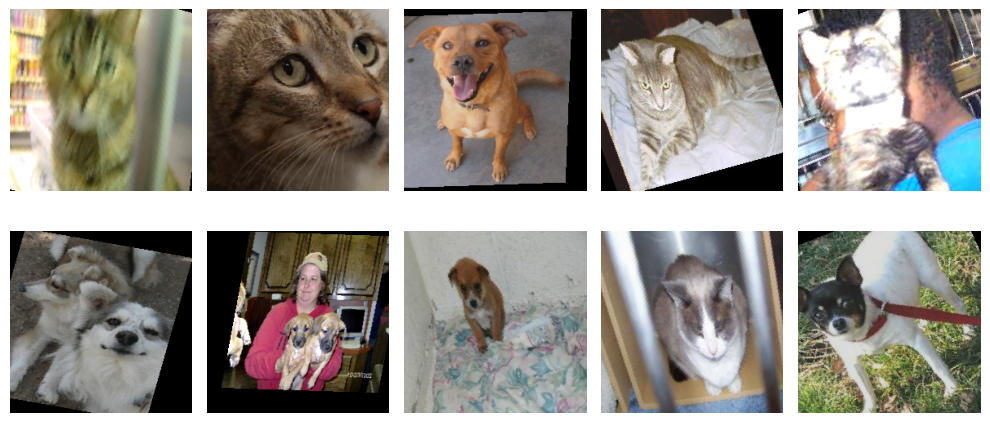
\includegraphics[width=0.5\textwidth]{figures/augmentation.png}}
    \caption{Data augmentation techniques.}
    \label{fig:augmentation}
    \vspace*{-0.7cm}
\end{figure}


\begin{figure}[H]
    \centering
    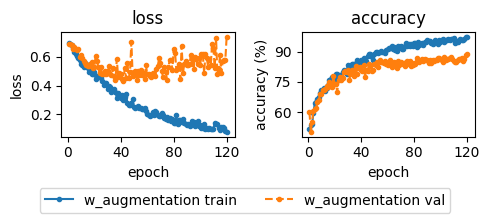
\includegraphics[width=0.4\textwidth]{figures/results_augmentation.png}
    \caption{Sample images after augmentation.}
    \label{fig:augmentation_results}
\end{figure}


\subsection{More Regularization Techniques}


1:
- 93% valideringsæt
- 84% test

2:
- 93% valideringsæt
- 85% test sæt

- loss mere stabil på 2. Den er med weight decay og halvering af learning rate hver 25 epoker.
- dropout layer

\begin{figure}[H]
    \vspace*{-0.7cm}
    \centering
    \subfloat[Regularized model 1.\label{fig:reg1}]{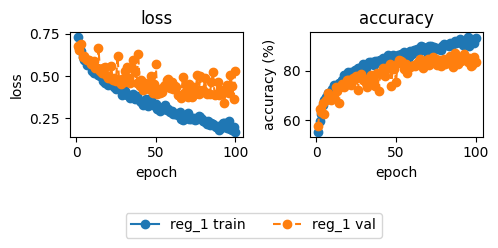
\includegraphics[width=0.4\textwidth]{figures/results_reg_1.png}}
    \hspace{1cm}
    \subfloat[Regularized model 2.\label{fig:reg2}]{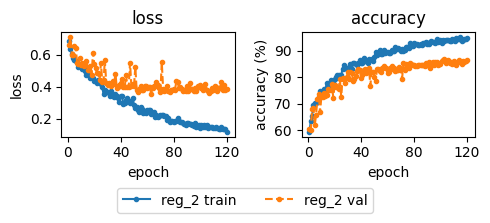
\includegraphics[width=0.4\textwidth]{figures/results_reg_2.png}}
    \caption{Results using regularization.}
    \label{fig:reg}
    \vspace*{-0.7cm}
\end{figure}

\subsection{Adding one more convolutional layer}
\begin{figure}[H]
    \vspace*{-0.7cm}
    \centering
    \subfloat[Regularized model 3.\label{fig:reg1}]{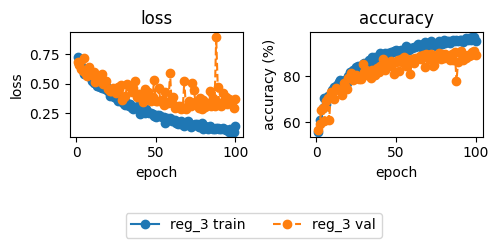
\includegraphics[width=0.4\textwidth]{figures/results_reg_3.png}}
    \hspace{1cm}
    \subfloat[Regularized model 4.\label{fig:reg2}]{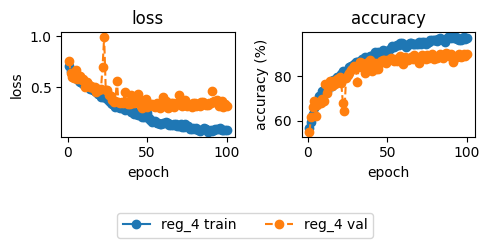
\includegraphics[width=0.4\textwidth]{figures/results_reg_4.png}}
    \caption{Results using one more convolutional layer.}
    \label{fig:reg}
    \vspace*{-0.7cm}
\end{figure}